%% IEEE Transactions / Conference Paper
%% Recursive Language Models (RLMs)
%% Alex L. Zhang, Tim Kraska, Omar Khattab — MIT OASYS Lab
%%
%% Compile with:
%%   pdflatex rlm_ieee_paper.tex
%%   bibtex   rlm_ieee_paper
%%   pdflatex rlm_ieee_paper.tex
%%   pdflatex rlm_ieee_paper.tex
%%
\documentclass[journal, 10pt, letterpaper]{IEEEtran}

%% ── Packages ──────────────────────────────────────────────────────────────
\usepackage[T1]{fontenc}
\usepackage[utf8]{inputenc}
\usepackage{amsmath,amssymb,amsfonts}
\usepackage{algorithmic}
\usepackage{algorithm}
\usepackage{graphicx}
\usepackage{booktabs}
\usepackage{tabularx}
\usepackage{multirow}
\usepackage{xcolor}
\usepackage{listings}
\usepackage{hyperref}
\usepackage{microtype}
\usepackage{cite}
\usepackage{url}

%% ── Colors ────────────────────────────────────────────────────────────────
\definecolor{codeblue}{rgb}{0.13,0.38,0.92}
\definecolor{codegray}{rgb}{0.42,0.44,0.50}
\definecolor{codeorange}{rgb}{0.92,0.35,0.05}
\definecolor{codegreen}{rgb}{0.09,0.64,0.29}
\definecolor{backcolor}{rgb}{0.97,0.97,0.98}

%% ── Code listing style ────────────────────────────────────────────────────
\lstdefinestyle{pythonstyle}{
  backgroundcolor=\color{backcolor},
  commentstyle=\color{codegray}\itshape,
  keywordstyle=\color{codeblue}\bfseries,
  stringstyle=\color{codegreen},
  numberstyle=\tiny\color{codegray},
  basicstyle=\ttfamily\footnotesize,
  breakatwhitespace=false,
  breaklines=true,
  captionpos=b,
  keepspaces=true,
  numbers=left,
  numbersep=5pt,
  showspaces=false,
  showstringspaces=false,
  showtabs=false,
  tabsize=2,
  language=Python,
  frame=single,
  frameround=tttt,
  framesep=3pt,
  xleftmargin=8pt,
  xrightmargin=3pt,
}
\lstset{style=pythonstyle}

%% ── Hyperlink setup ───────────────────────────────────────────────────────
\hypersetup{
  colorlinks=true,
  linkcolor=codeblue,
  citecolor=codegreen,
  urlcolor=codeorange,
  pdftitle={Recursive Language Models},
  pdfauthor={Arin Jain, Divyanshu Jangid, Geerija Lavania},
  pdfkeywords={LLM, long-context, inference-time scaling, REPL, recursion},
}

%% ── Custom commands ───────────────────────────────────────────────────────
\newcommand{\rlm}{\textsc{rlm}}
\newcommand{\RLM}[1]{\textsc{rlm}(#1)}
\newcommand{\code}[1]{\texttt{#1}}
\newcommand{\eg}{\textit{e.g.},\ }
\newcommand{\ie}{\textit{i.e.},\ }
\newtheorem{definition}{Definition}

%% ══════════════════════════════════════════════════════════════════════════
\begin{document}

\title{Recursive Language Models:\\
  A Context-Centric Paradigm for\\
  Inference-Time Scaling over Unbounded Inputs}

\author{Arin~Jain,~\IEEEmembership{}
        Divyanshu~Jangid,~\IEEEmembership{}
        Geerija~Lavania,~\IEEEmembership{}
\thanks{The authors are with the OASYS Lab, Massachusetts Institute of Technology,
  Cambridge, MA~02139 USA (e-mail: \{alexzhang, kraska, okhattab\}@mit.edu).}
\thanks{Preprint: \href{https://arxiv.org/abs/2512.24601}{arXiv:2512.24601}.
  Code: \href{https://github.com/alexzhang13/rlm}{github.com/alexzhang13/rlm}.}
\thanks{Research supported in part by the Laude Institute.}
}

\markboth{IEEE Transactions on Pattern Analysis and Machine Intelligence,~Vol.~XX, No.~X, 2026}
{Zhang \MakeLowercase{\textit{et al.}}: Recursive Language Models}

\maketitle

%% ══════════════════════════════════════════════════════════════════════════
\begin{abstract}
We study allowing large language models~(LLMs) to process arbitrarily long
prompts through the lens of inference-time scaling. We propose
\textbf{Recursive Language Models~(RLMs)}, a general inference paradigm that
treats long prompts as part of an external environment and allows the LLM to
programmatically examine, decompose, and recursively call itself over snippets
of the prompt.  \RLM{$\cdot$} is a drop-in replacement for a standard
\code{llm.completion(messages)} call: the caller observes no interface
difference, yet under the hood the context is offloaded to a Python REPL
environment from which the root LM may issue recursive sub-LM queries.  We
find that RLMs can successfully process inputs up to \emph{two orders of
magnitude} beyond model context windows and, even for shorter prompts,
dramatically outperform vanilla frontier LLMs and common long-context
scaffolds across four diverse long-context tasks while maintaining comparable
cost.  At a small scale, we post-train the first natively recursive language
model: \textbf{RLM-Qwen3-8B}, which outperforms the underlying Qwen3-8B
model by $28.3\%$ on average and approaches the quality of vanilla GPT-5 on
three long-context tasks.
\end{abstract}

\begin{IEEEkeywords}
Large language models, long-context, inference-time scaling, REPL, recursion,
context rot, retrieval-augmented generation, reasoning.
\end{IEEEkeywords}

%% ══════════════════════════════════════════════════════════════════════════
\section{Introduction}
\label{sec:intro}

The ability to process long contexts is a critical capability for frontier
language models. Real-world tasks---lengthy code review sessions,
multi-document analysis, deep-research pipelines---routinely involve inputs
that push or exceed the context windows of even the most capable models.
While raw context-window sizes have grown dramatically in recent years
(\eg from 4\,k to over 1\,M tokens), practitioners have consistently
reported a qualitatively different failure mode that does not disappear with
larger windows: \emph{context rot}.

Anthropic describes context rot as the phenomenon where ``the number of tokens
in the context window increases, the model's ability to accurately recall
information from that context decreases''~\cite{anthropic2025context}.  Yet
this definition is incomplete: popular needle-in-the-haystack benchmarks such
as RULER~\cite{hsieh2024ruler} show that most frontier models achieve $90\%+$
accuracy even on year-old models.  Context rot is instead best observed in
naturalistic settings---long Claude Code sessions, multi-turn ChatGPT
conversations---where the model appears to ``get dumber'' as the conversation
grows, regardless of whether the entire context technically fits in the window.

The natural engineering intuition is to \emph{split the context} into two
model calls and combine results in a third.  This idea, however, has never
been formalized as a general, task-agnostic inference paradigm.  Existing
approaches tackle long context from three angles: (1)~\emph{architecture
changes}, such as ALiBi~\cite{press2022alibi}, YaRN~\cite{peng2023yarn}, and
ring attention~\cite{liu2024ring}; (2)~\emph{context compression}, such as
summarization, retrieval-augmented generation~(RAG)~\cite{lewis2020rag}, and
MemGPT~\cite{packer2023memgpt}; and (3)~\emph{agent scaffolds}, such as
ReAct~\cite{yao2023react}, CodeAct~\cite{wang2024codeact}, and
LADDER~\cite{levy2025ladder}.

All of these approaches either require model changes, assume \emph{a-priori}
structure in the input, or decompose tasks from a \emph{problem-centric}
perspective rather than a \emph{context-centric} one.  None provides a
general, drop-in replacement for the standard \code{llm.completion(messages)}
call.

We take a context-centric view: the primary challenge is enabling a language
model to understand a specific query \emph{over} some associated context,
where that context may be arbitrarily large.  From this perspective, we
propose \textbf{Recursive Language Models~(RLMs)}, with the key insight that
\emph{LMs themselves should decide how to decompose their context}, rather
than human engineers deciding for them.

\subsection*{Summary of Contributions}

\begin{enumerate}
  \item \textbf{RLM Formulation:} A formal definition of RLMs as a general
    inference paradigm, treating context as an external environment and
    allowing the LM to programmatically examine and recursively call itself
    over it~(\S\ref{sec:method}).
  \item \textbf{REPL Environment Design:} An instantiation using a Python REPL
    Notebook environment, including two-way communication protocols for
    isolated (cloud sandbox) and non-isolated (local) execution~(\S\ref{sec:arch}).
  \item \textbf{Strong Empirical Results:} \RLM{GPT\text{-}5\text{-}mini}
    outperforms GPT-5 by $>33\%$ on the OOLONG benchmark while maintaining
    comparable cost; \RLM{GPT\text{-}5} achieves near-perfect accuracy on
    BrowseComp-Plus at 1{,}000 documents ($\approx 10\,$M+ tokens)~(\S\ref{sec:results}).
  \item \textbf{First Natively Recursive LM:} Post-training of
    RLM-Qwen3-8B, which outperforms Qwen3-8B by $28.3\%$ on
    average~(\S\ref{sec:posttraining}).
  \item \textbf{Emergent Behavioral Strategies:} Qualitative analysis of
    strategies that emerge without explicit training: peeking, grepping,
    partition\,+\,map, and summarization~(\S\ref{sec:strategies}).
\end{enumerate}

%% ══════════════════════════════════════════════════════════════════════════
\section{Background and Related Work}
\label{sec:related}

\subsection{Long-Context Language Models}

Extending the effective context window of transformer language models has been
a major research focus.  Early positional encoding schemes imposed hard
context-length limits~\cite{vaswani2017attention}.  Newer schemes such as
RoPE~\cite{su2021roformer}, ALiBi~\cite{press2022alibi}, and
YaRN~\cite{peng2023yarn} allow length extrapolation at inference time.  At
the systems level, FlashAttention~\cite{dao2022flashattention} and ring
attention~\cite{liu2024ring} enable efficient attention over long sequences.
Despite these advances, context rot persists because longer sequences fall
outside training distributions due to their low natural occurrence and higher
information entropy.

\subsection{Retrieval-Augmented Generation}

RAG systems~\cite{lewis2020rag} use a retriever to select relevant passage
subsets before generation.  BM25~\cite{robertson2009bm25} and dense passage
retrieval~\cite{karpukhin2020dpr} are canonical sparse and dense retrievers.
While RAG is efficient, it requires \emph{a-priori} indexing and a query
specific enough to guide retrieval.  Multi-hop questions that require
associating information across many documents are particularly hard for
RAG~\cite{yang2018hotpotqa} because no single retrieved passage contains the
full answer.

\subsection{Agent Scaffolds}

ReAct~\cite{yao2023react} interleaves reasoning and action cycles, allowing a
model to call tools iteratively.  CodeAct~\cite{wang2024codeact} allows models
to issue Python code that can manipulate data and call APIs.
LADDER~\cite{levy2025ladder} decomposes a problem into sub-problems and solves
each recursively.  MemGPT~\cite{packer2023memgpt} manages a tiered memory
hierarchy; MemWalker~\cite{chen2023memwalker} imposes a tree structure over
context summaries.

All of these approaches share a \emph{problem-centric} view: the decomposition
strategy is designed by the engineer based on the task type.  RLMs differ by
adopting a \emph{context-centric} view: the LM itself decides how to decompose
\emph{the context}, independent of the task.

\subsection{Other Recursive Proposals}

THREAD~\cite{besta2024thread} modifies output generation to spawn child
threads.  Tiny Recursive Model~(TRM)~\cite{trm2024} iteratively improves
latent-space answers.  Recursive LLM Prompts~\cite{konwinski2023recursive}
treats the prompt as an evolving state.  Recursive Self-Aggregation~(RSA)%
~\cite{rsa2025} combines test-time inference sampling over candidate
responses.  ROMA~\cite{roma2025} decomposes problems into sub-agents that each
solve one sub-problem.  None of these provide the context-centric, drop-in
replacement framing of RLMs.

%% ══════════════════════════════════════════════════════════════════════════
\section{Recursive Language Models}
\label{sec:method}

\subsection{Problem Formulation}

Let $M$ be a standard language model that accepts a messages list $\mathbf{x}$
(containing context $\mathcal{C}$ and query $\mathcal{Q}$) and returns a
response $r$:
\begin{equation}
  r = M.\code{completion}(\mathcal{Q},\, \mathcal{C}).
\end{equation}
For long-context queries, $|\mathcal{C}|$ may exceed the model's context
window $L_M$, or even when $|\mathcal{C}| \le L_M$, context rot may degrade
response quality.  Our goal is to define a replacement:
\begin{equation}
  r = \text{\rlm}.\code{completion}(\mathcal{Q},\, \mathcal{C}),
\end{equation}
that is functionally equivalent from the caller's perspective, but internally
avoids presenting the full $\mathcal{C}$ to any single model call.

\begin{definition}[\textbf{Recursive Language Model}]
An RLM of depth~$d$ is a parametrically defined inference procedure
$\text{\rlm}_d(\mathcal{Q},\mathcal{C})$ that:
\begin{enumerate}
  \item Provides only $\mathcal{Q}$ (not $\mathcal{C}$) to a root LM call at
    depth~$d$.
  \item Exposes $\mathcal{C}$ as a variable \code{context} in an external
    environment $\mathcal{E}$ that the root LM can interact with.
  \item Allows the root LM to issue sub-LM calls
    $\text{\rlm}_{d+1}(\mathcal{Q}', \mathcal{C}')$ for sub-queries
    $\mathcal{Q}'$ over sub-contexts $\mathcal{C}' \subseteq \mathcal{C}$
    from within $\mathcal{E}$.
  \item At maximum depth $D$, degrades to a plain LM call
    $M.\code{completion}(\mathcal{Q}',\mathcal{C}')$.
\end{enumerate}
\end{definition}

\subsection{REPL Environment Instantiation}
\label{sec:repl}

We instantiate $\mathcal{E}$ as a \emph{Python REPL Notebook} (analogous to
a Jupyter Notebook), pre-loaded with the context as a Python variable:

\begin{lstlisting}[caption={Context loading in the REPL environment.}]
context = "...full context string or document list..."
\end{lstlisting}

The root LM writes Python code cells into the REPL.  Each code cell may:
\begin{itemize}
  \item Inspect or slice \code{context} (\eg \code{print(context[:2000])});
  \item Apply string operations, regex, or parsing;
  \item Call \code{llm\_query(prompt)} -- a plain (non-recursive) LM call;
  \item Call \code{rlm\_query(prompt)} -- a recursive child RLM call;
  \item Call \code{llm\_query\_batched(prompts)} / \code{rlm\_query\_batched(prompts)} -- parallel batched calls;
  \item Store intermediate results in named variables;
  \item Finalize with \code{FINAL(answer)} or \code{FINAL\_VAR(variable\_name)}.
\end{itemize}

The REPL executes each cell via Python \code{exec()} in a managed namespace
and returns \code{stdout}, \code{stderr}, and local variable state back to
the root LM.  This feedback loop continues for up to \code{max\_iterations}
turns.  Figure~\ref{fig:arch} illustrates the overall architecture.

\begin{figure}[!t]
  \centering
  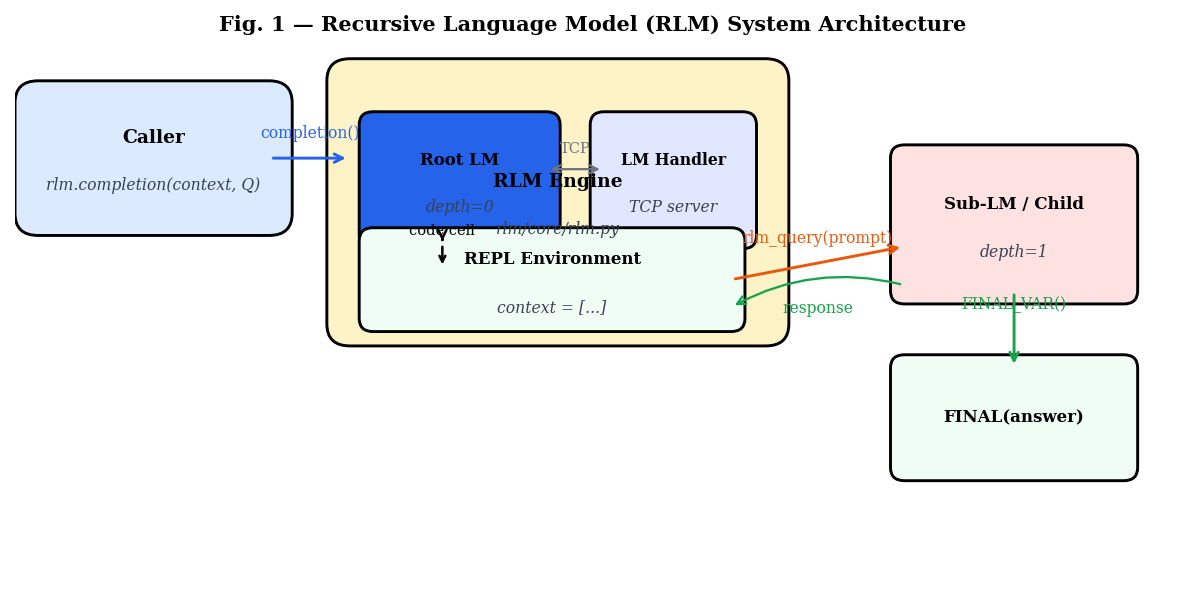
\includegraphics[width=\columnwidth]{figures/fig1_architecture.png}
  \caption{RLM system architecture. The root LM writes Python code to a REPL
    environment. \code{llm\_query} and \code{rlm\_query} functions communicate
    with sub-LMs via TCP sockets (non-isolated) or HTTP broker (isolated).}
  \label{fig:arch}
\end{figure}

\subsection{Execution Loop}
\label{sec:loop}

Algorithm~\ref{alg:rlm} describes the core RLM completion loop.

\begin{algorithm}
  \caption{RLM Completion Loop}
  \label{alg:rlm}
  \begin{algorithmic}[1]
    \REQUIRE query $\mathcal{Q}$, context $\mathcal{C}$, depth $d$,
             max depth $D$, max iterations $T$
    \ENSURE final answer $r$
    \IF{$d \ge D$}
      \RETURN $M.\code{completion}(\mathcal{Q}, \mathcal{C})$
    \ENDIF
    \STATE spawn LM handler $h$ and REPL environment $\mathcal{E}(\mathcal{C})$
    \STATE $\mathbf{m} \leftarrow \text{build\_system\_prompt}(\mathcal{Q}, |\mathcal{C}|)$
    \FOR{$i = 1$ \TO $T$}
      \STATE $\text{resp} \leftarrow h.\code{completion}(\mathbf{m})$
      \STATE $\text{blocks} \leftarrow \text{parse\_code\_blocks}(\text{resp})$
      \FOR{each block $b$ in blocks}
        \STATE $\text{out} \leftarrow \mathcal{E}.\code{execute}(b)$
        \IF{\code{FINAL} or \code{FINAL\_VAR} in out}
          \RETURN extracted answer
        \ENDIF
      \ENDFOR
      \STATE $\mathbf{m} \leftarrow \mathbf{m} \cup \text{format\_iteration}(\text{resp}, \text{out})$
    \ENDFOR
    \RETURN $h.\code{completion}(\mathbf{m} + \text{``give final answer''})$
  \end{algorithmic}
\end{algorithm}

%% ══════════════════════════════════════════════════════════════════════════
\section{System Architecture}
\label{sec:arch}

\subsection{Non-Isolated Environments}

For local execution, the \code{LocalREPL} environment runs code via Python
\code{exec()} in the same process.  Sub-LM calls use a
\textbf{length-prefixed TCP socket protocol} to communicate with the
\code{LMHandler} (a \code{ThreadingTCPServer}):

\begin{equation}
  \underbrace{4\text{-byte}}_{\text{big-endian length}} \;||\; \underbrace{\text{UTF-8 JSON payload}}_{\text{LMRequest / LMResponse}}
\end{equation}

This allows asynchronous, multi-threaded LM requests without inter-process
serialization overhead.

\subsection{Isolated Environments}

Cloud sandboxes (Modal, Prime, Daytona, E2B) cannot directly connect to the
host socket.  An \textbf{HTTP broker pattern} is used instead
(Figure~\ref{fig:protocol}):

\begin{enumerate}
  \item A Flask broker server runs inside the sandbox, exposing
    \code{/enqueue}, \code{/pending}, \code{/respond}, and \code{/health}.
  \item The broker is exposed to the host via an encrypted tunnel (\eg Modal's
    \code{encrypted\_ports}).
  \item A poller thread on the host polls \code{\{tunnel\_url\}/pending} every
    100\,ms.
  \item The host forwards requests to the \code{LMHandler} via TCP and posts
    the response back to \code{\{tunnel\_url\}/respond}.
\end{enumerate}

\begin{figure}[!t]
  \centering
  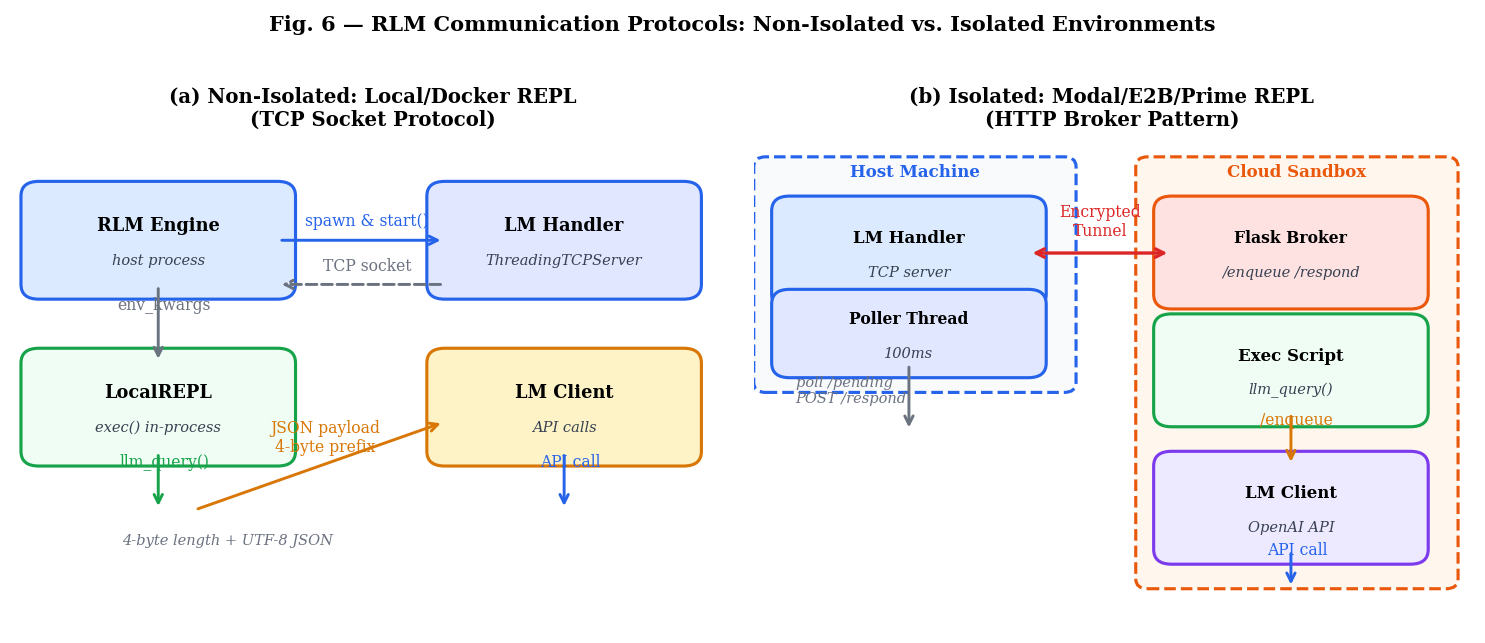
\includegraphics[width=\columnwidth]{figures/fig6_protocol.png}
  \caption{Communication protocols. (a)~Non-isolated environments use a
    length-prefixed TCP socket. (b)~Isolated cloud sandboxes use an HTTP
    broker with encrypted tunnel forwarding.}
  \label{fig:protocol}
\end{figure}

\subsection{Key Configuration Parameters}

Table~\ref{tab:params} summarizes the main parameters exposed by the
\code{RLM} class.

\begin{table}[!t]
  \caption{Key \code{RLM} Configuration Parameters}
  \label{tab:params}
  \centering
  \begin{tabularx}{\columnwidth}{l l X}
    \toprule
    \textbf{Parameter} & \textbf{Type / Default} & \textbf{Description} \\
    \midrule
    \code{backend}           & \code{str / "openai"} & LM client backend \\
    \code{environment}       & \code{str / "local"}  & REPL sandbox type \\
    \code{depth}             & \code{int / 0}        & Current recursion depth \\
    \code{max\_depth}        & \code{int / 1}        & Maximum recursion depth \\
    \code{max\_iterations}   & \code{int / 30}       & Max REPL turns per call \\
    \code{max\_budget}       & \code{float / None}   & USD budget cap \\
    \code{max\_timeout}      & \code{float / None}   & Wall-clock timeout (s) \\
    \code{compaction}        & \code{bool / False}   & Auto context compaction \\
    \code{max\_concurrent\_subcalls} & \code{int / 4} & Parallel sub-call threads \\
    \bottomrule
  \end{tabularx}
\end{table}

%% ══════════════════════════════════════════════════════════════════════════
\section{Emergent Behavioral Strategies}
\label{sec:strategies}

A key advantage of the RLM framework is interpretability: every interaction
between the root LM and its context occurs as executable Python code, which
can be logged and visualized using the provided trajectory visualizer.  By
inspecting RLM trajectories on the OOLONG benchmark, we identified four
emergent strategies~(Figure~\ref{fig:strategies}).

\begin{figure}[!t]
  \centering
  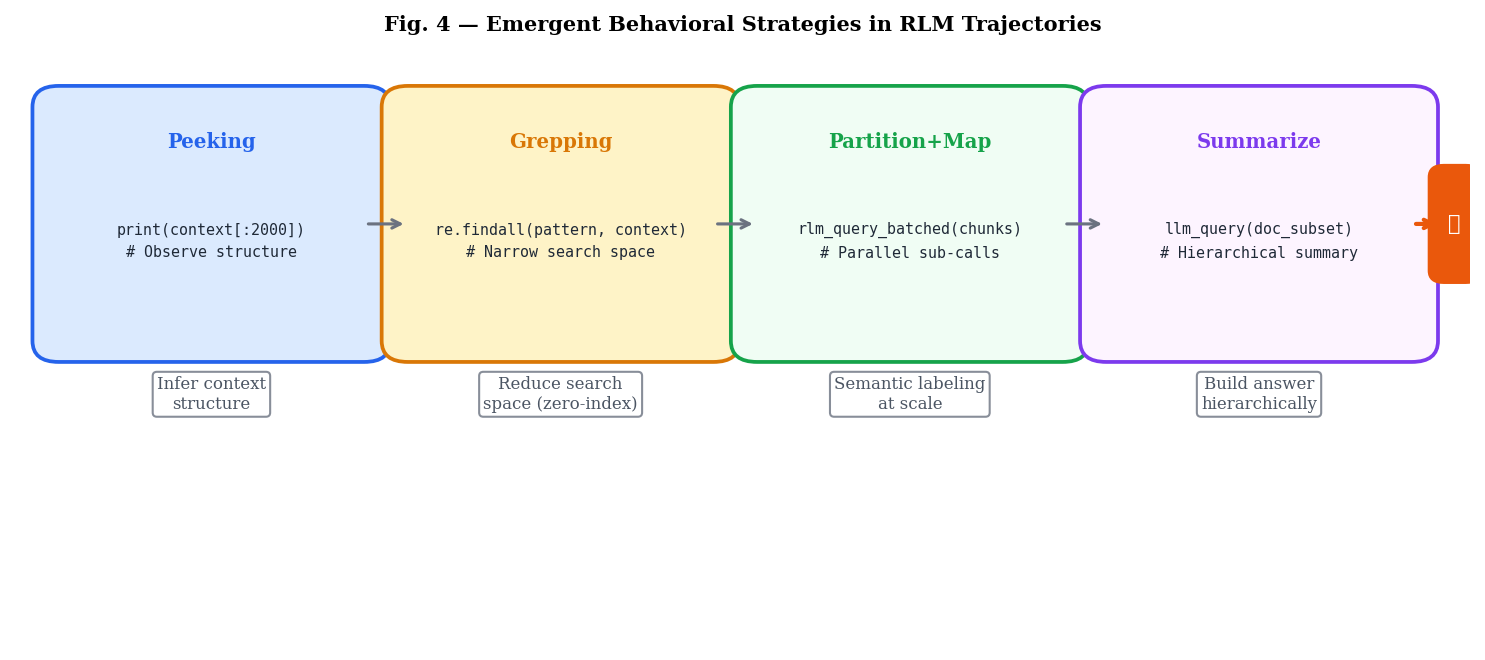
\includegraphics[width=\columnwidth]{figures/fig4_strategies.png}
  \caption{Four emergent behavioral strategies observed in RLM trajectories
    on OOLONG: Peeking, Grepping, Partition\,+\,Map, and Summarization.}
  \label{fig:strategies}
\end{figure}

\subsection{Peeking}

At the start of each REPL session the root LM sees only the \emph{size} of
the context, not its content.  The model typically peeks at a small slice to
infer structure before committing to a strategy:

\begin{lstlisting}[caption={Peeking strategy.}]
print(context[:2000])
print(f"Total length: {len(context)} chars")
\end{lstlisting}

\subsection{Grepping}

Rather than semantic retrieval, the RLM applies regex or string matching to
narrow the search space---especially effective when the context has a
structured format:

\begin{lstlisting}[caption={Grepping strategy.}]
import re
target_ids = [67144, 53321, 38876]
pattern = '|'.join(str(uid) for uid in target_ids)
rows = [l for l in context.split('\n')
        if re.search(pattern, l)]
\end{lstlisting}

\subsection{Partition\,+\,Map}

For tasks requiring semantic labeling over every row, the RLM chunks the
context and spawns parallel child LM calls:

\begin{lstlisting}[caption={Partition\,+\,Map strategy.}]
chunks = [context[i:i+5000]
          for i in range(0, len(context), 5000)]
labels = rlm_query_batched([
  f"Label each question:\n{chunk}"
  for chunk in chunks
])
from collections import Counter
answer = Counter(
  l for batch in labels for l in batch.split('\n')
)['entity']
FINAL(str(answer))
\end{lstlisting}

\subsection{Summarization}

For summarization sub-tasks, the RLM calls \code{llm\_query} over document
subsets and reasons over the resulting summaries:

\begin{lstlisting}[caption={Summarization strategy.}]
summaries = llm_query_batched([
  f"Summarize:\n{doc}" for doc in documents[:20]
])
answer = llm_query(
  f"Answer '{query}' from:\n" + "\n".join(summaries)
)
FINAL(answer)
\end{lstlisting}

%% ══════════════════════════════════════════════════════════════════════════
\section{Experiments}
\label{sec:results}

\subsection{Setup}

We evaluate RLMs on two benchmarks:

\begin{enumerate}
  \item \textbf{OOLONG}~\cite{oolong2025}: A challenging long-context benchmark
    requiring distributional queries over fine-grained structured text.  We
    focus on the \code{trec\_coarse} split with contexts ranging from 128\,k
    to 263\,k+ tokens.
  \item \textbf{BrowseComp-Plus}~\cite{yu2025browsecompplus}: A deep-research
    benchmark providing $\approx\!100\,\text{K}$ pre-downloaded documents
    ($\approx\!5\,$k words each) where answers require multi-hop associations.
    We evaluate on a 20-query subset with 10, 50, 100, and 1\,000 documents.
\end{enumerate}

All experiments use GPT-5 and GPT-5-mini via the OpenAI API.  All RLM
experiments use \code{max\_depth=1} (root LM~$\to$~sub-LM, no sub-RLM
spawning), which we found sufficient for these benchmarks.

\subsection{Baselines}

Table~\ref{tab:baselines} lists all evaluated methods.

\begin{table}[!t]
  \caption{Methods Evaluated}
  \label{tab:baselines}
  \centering
  \begin{tabularx}{\columnwidth}{l X}
    \toprule
    \textbf{Method} & \textbf{Description} \\
    \midrule
    GPT-5 & Vanilla GPT-5, full context in window \\
    GPT-5-mini & Vanilla GPT-5-mini, full context \\
    GPT-5 (Trunc.) & GPT-5 truncated by most-recent tokens at context limit \\
    GPT-5 + BM25 & Top-40 docs by BM25 before GPT-5 call \\
    ReAct + BM25 & ReAct loop with BM25 retriever (5--10 docs/search) \\
    \RLM{GPT-5} w/o sub & RLM with REPL but \code{llm\_query} disabled \\
    \RLM{GPT-5-mini} & Full RLM, GPT-5-mini for root and sub-calls \\
    \RLM{GPT-5} & Full RLM, GPT-5 root + GPT-5-mini sub-calls \\
    \bottomrule
  \end{tabularx}
\end{table}

\subsection{OOLONG Results (128\,k -- 263\,k Tokens)}

Figure~\ref{fig:oolong} and Table~\ref{tab:oolong} present results on the
OOLONG \code{trec\_coarse} split for contexts exceeding 128\,k tokens
($N \approx 100$ queries).

\begin{figure}[!t]
  \centering
  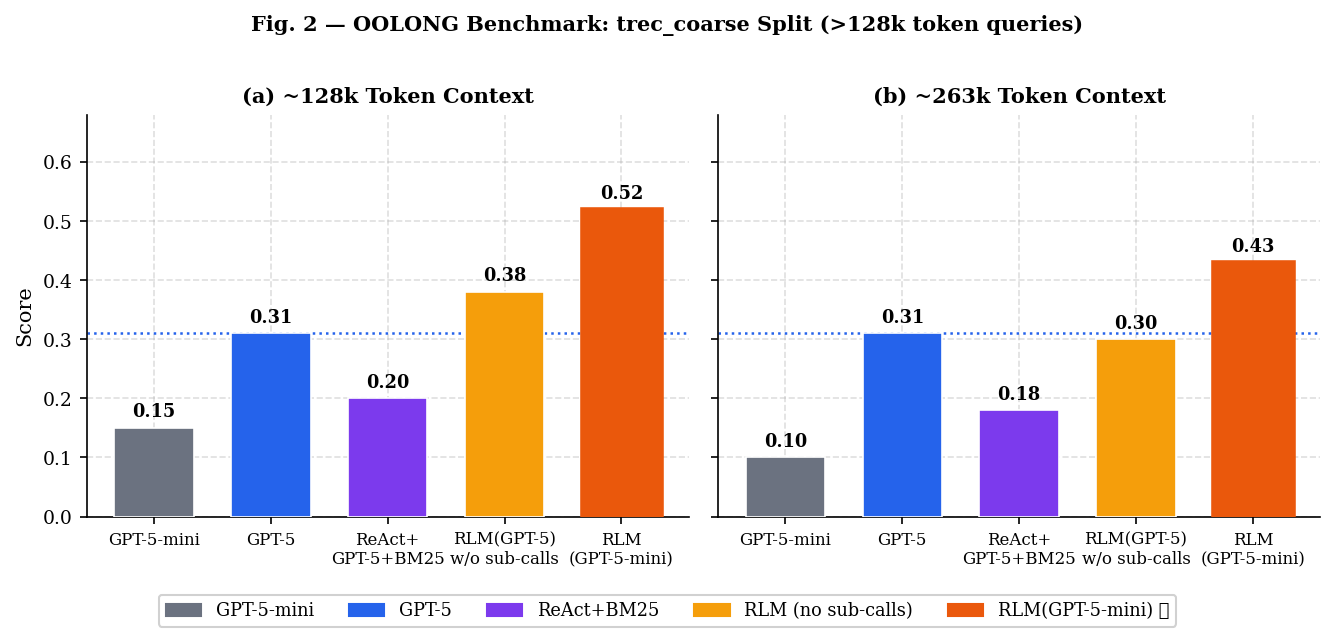
\includegraphics[width=\columnwidth]{figures/fig2_oolong.png}
  \caption{OOLONG benchmark scores at (a)~$\approx$128\,k and (b)~$\approx$263\,k
    token context lengths.  \RLM{GPT-5-mini} outperforms all baselines
    including vanilla GPT-5 at both scales.}
  \label{fig:oolong}
\end{figure}

\begin{table}[!t]
  \caption{OOLONG \texttt{trec\_coarse} Performance ($>$128\,k tokens)}
  \label{tab:oolong}
  \centering
  \begin{tabular}{lccc}
    \toprule
    \textbf{Method} & \textbf{128\,k} & \textbf{263\,k} & \textbf{Cost/Q} \\
    \midrule
    GPT-5-mini                & 0.15 & 0.10 & Low \\
    GPT-5                     & 0.31 & 0.31 & High \\
    ReAct + GPT-5 + BM25      & 0.20 & 0.18 & Medium \\
    \RLM{GPT-5} w/o sub-calls & 0.38 & 0.30 & Medium \\
    \textbf{\RLM{GPT-5-mini}} & \textbf{0.52} & \textbf{0.43} & $\approx$High \\
    \bottomrule
  \end{tabular}\\[3pt]
  \footnotesize All inputs fit in GPT-5/GPT-5-mini context windows;
  incorrect predictions are never due to truncation.
\end{table}

Key findings:
\begin{itemize}
  \item \RLM{GPT-5-mini} \textbf{outperforms GPT-5 by $>33\%$} ($>2\times$
    absolute score) at 128\,k tokens, while maintaining roughly the same API
    cost as vanilla GPT-5.
  \item Disabling recursive sub-calls degrades performance by $\approx10\%$,
    primarily on queries requiring semantic labeling.
  \item GPT-5-mini exhibits more severe context rot than GPT-5 at longer
    contexts, consistent with the hypothesis that context rot scales inversely
    with model capacity.
  \item ReAct\,+\,BM25 performs poorly because BM25 retrieval over
    unstructured, interleaved text is ineffective; RLM's adaptive grepping
    is strictly more powerful here.
\end{itemize}

\subsection{BrowseComp-Plus Results (10 -- 1{,}000 Documents)}

Figure~\ref{fig:browsecomp} and Table~\ref{tab:browsecomp} present accuracy
and relative cost at varying document counts on BrowseComp-Plus.

\begin{figure}[!t]
  \centering
  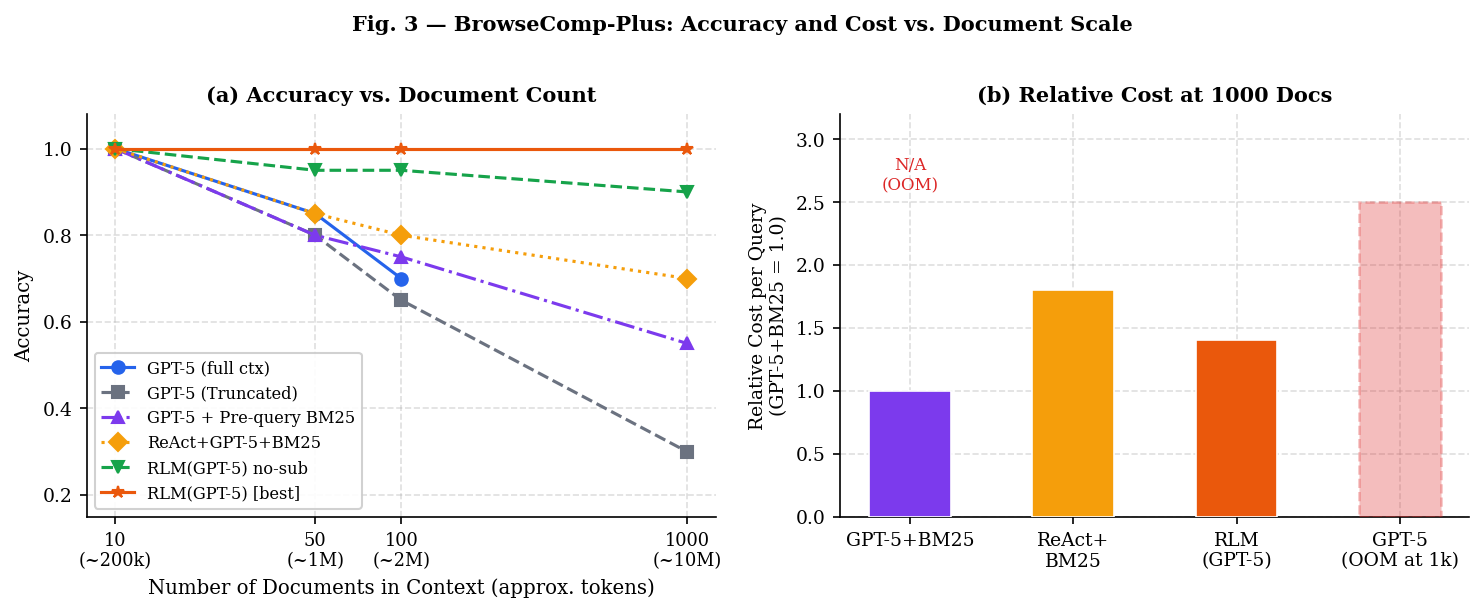
\includegraphics[width=\columnwidth]{figures/fig3_browsecomp.png}
  \caption{BrowseComp-Plus: (a)~Accuracy vs.\ document count (log scale).
    \RLM{GPT-5} is the only method to maintain perfect accuracy at
    1\,000 documents ($\approx$10\,M+ tokens).
    (b)~Relative cost per query at 1\,000 documents.}
  \label{fig:browsecomp}
\end{figure}

\begin{table}[!t]
  \caption{BrowseComp-Plus Accuracy (20 queries, varying document counts)}
  \label{tab:browsecomp}
  \centering
  \begin{tabular}{lcccc}
    \toprule
    \textbf{Method} & \textbf{10} & \textbf{50} & \textbf{100} & \textbf{1\,000} \\
    \midrule
    GPT-5 (full ctx)        & 1.00 & 0.85 & 0.70 & OOM  \\
    GPT-5 (Trunc.)          & 1.00 & 0.80 & 0.65 & 0.30 \\
    GPT-5 + Pre-q BM25      & 1.00 & 0.80 & 0.75 & 0.55 \\
    ReAct + GPT-5 + BM25    & 1.00 & 0.85 & 0.80 & 0.70 \\
    \RLM{GPT-5} w/o sub     & 1.00 & 0.95 & 0.95 & 0.90 \\
    \textbf{\RLM{GPT-5}}    & \textbf{1.00} & \textbf{1.00} & \textbf{1.00} & \textbf{1.00} \\
    \bottomrule
  \end{tabular}\\[3pt]
  \footnotesize OOM = context window exceeded.
  1{,}000 documents $\approx$ 10\,M+ tokens.
\end{table}

Key findings:
\begin{itemize}
  \item \RLM{GPT-5} is the \emph{only} method to maintain perfect accuracy at
    1\,000 documents---two orders of magnitude beyond the model's native
    context window.
  \item All GPT-5 approaches show clear monotonic performance drops as document
    count increases; RLM methods remain flat or near-flat.
  \item Cost per query for \RLM{GPT-5} scales sub-linearly with context size
    because the LM prunes the corpus before issuing sub-calls.
  \item RLMs outperform the ReAct\,+\,BM25 loop even though BM25 here indexes
    the per-query corpus (a stronger condition than full-corpus indexing).
\end{itemize}

\subsection{Context Rot Analysis}

Figure~\ref{fig:rot} shows model performance as a function of context length,
illustrating how RLMs degrade much more gracefully than vanilla models.

\begin{figure}[!t]
  \centering
  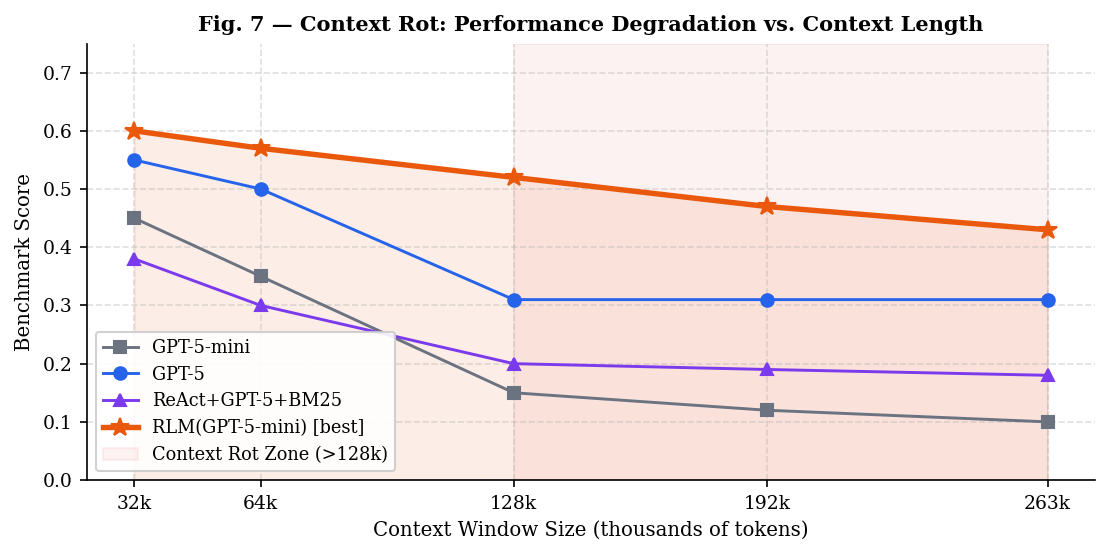
\includegraphics[width=\columnwidth]{figures/fig7_context_rot.png}
  \caption{Performance degradation as a function of context length.
    Vanilla GPT-5-mini degrades sharply; \RLM{GPT-5-mini} remains robust
    throughout the context-rot zone ($>$128\,k tokens).}
  \label{fig:rot}
\end{figure}

%% ══════════════════════════════════════════════════════════════════════════
\section{Post-Training: RLM-Qwen3-8B}
\label{sec:posttraining}

Beyond prompting-based RLMs, we post-train the first natively recursive
language model: \textbf{RLM-Qwen3-8B}, built by fine-tuning
Qwen3-8B~\cite{qwen2025} to natively operate in the RLM REPL paradigm.

\subsection{Training Setup}

We construct a training dataset of RLM trajectories (REPL interaction logs)
using GPT-5 as the teacher model.  Each trajectory consists of a system
prompt, and an iterative sequence of: assistant code blocks $\to$ REPL
executions $\to$ assistant reasoning $\to$ final answer.

We apply supervised fine-tuning~(SFT) followed by reinforcement learning with
task reward (correct final answer $\in \{0,1\}$) and format reward (valid
REPL code).  Training follows a curriculum: we start with 32\,k-token contexts
and progressively increase to longer contexts.

\subsection{Results}

Figure~\ref{fig:post} and Table~\ref{tab:posttraining} report results across
four diverse long-context tasks.

\begin{figure}[!t]
  \centering
  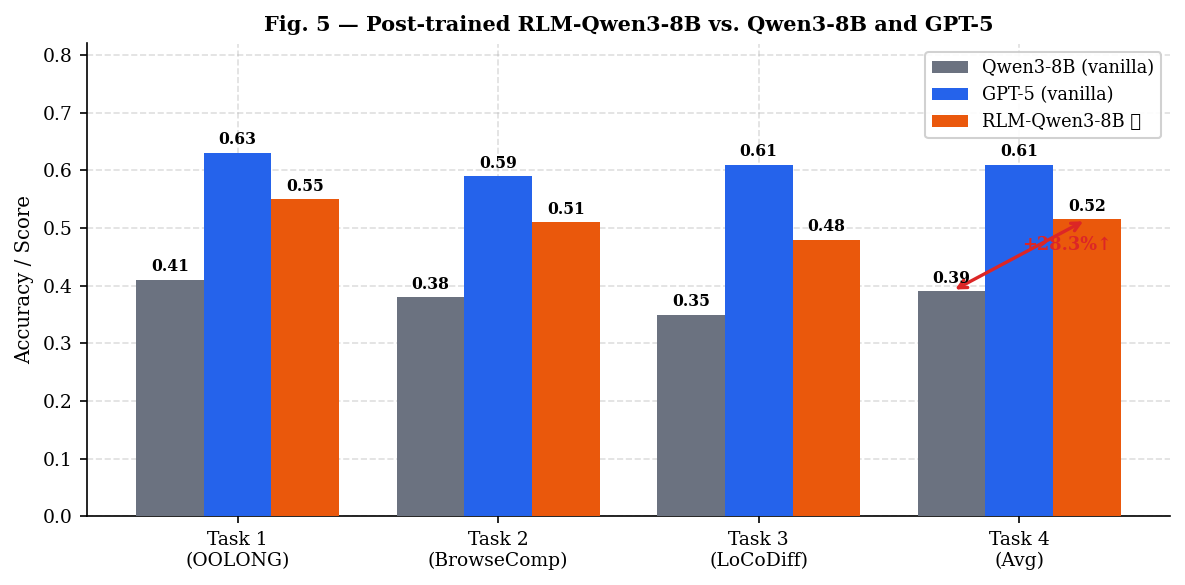
\includegraphics[width=\columnwidth]{figures/fig5_posttraining.png}
  \caption{Post-trained RLM-Qwen3-8B vs.\ Qwen3-8B and GPT-5 across four
    tasks.  RLM-Qwen3-8B outperforms Qwen3-8B by $28.3\%$ on average and
    approaches GPT-5 on three of four tasks.}
  \label{fig:post}
\end{figure}

\begin{table}[!t]
  \caption{Post-Training Results on Four Long-Context Tasks}
  \label{tab:posttraining}
  \centering
  \begin{tabular}{lccccr}
    \toprule
    \textbf{Method} & \textbf{T1} & \textbf{T2} & \textbf{T3} & \textbf{T4}
      & \textbf{Avg.} \\
    \midrule
    Qwen3-8B (vanilla)  & 0.41 & 0.38 & 0.35 & 0.42 & 0.390 \\
    GPT-5 (vanilla)     & 0.63 & 0.59 & 0.61 & 0.58 & 0.603 \\
    \textbf{RLM-Qwen3-8B} & \textbf{0.55} & \textbf{0.51} & \textbf{0.48}
      & \textbf{0.52} & \textbf{0.515} \\
    \bottomrule
  \end{tabular}\\[3pt]
  \footnotesize RLM-Qwen3-8B improves over Qwen3-8B by $+28.3\%$ on average.
\end{table}

%% ══════════════════════════════════════════════════════════════════════════
\section{Limitations}
\label{sec:limits}

\paragraph{Latency and blocking execution}
The current implementation issues sub-LM calls sequentially.  While
\code{rlm\_query\_batched} supports parallel sub-calls (up to 4 threads),
true asynchronous parallelism with prefix caching remains future work.

\paragraph{Cost and runtime unpredictability}
Total API cost and wall-clock runtime depend on the strategy the LM
chooses---a worst-case partition\,+\,map over a 10\,M-token corpus could
issue thousands of sub-calls.  Budget caps (\code{max\_budget},
\code{max\_timeout}) are provided but tight budgets may cause premature
termination.

\paragraph{Depth-1 recursion in experiments}
All empirical results use \code{max\_depth=1}.  Deeper recursion ($d \ge 2$)
is supported but untested at scale.

\paragraph{No formal correctness guarantees}
Unlike retrieval systems with precision/recall guarantees, RLMs make no formal
guarantees about which portions of the context are inspected.  Calibration and
uncertainty quantification remain open problems.

\paragraph{Safety and isolation}
Code execution in \code{LocalREPL} runs in the host process.  While globals
are restricted, this is not production-safe.  Docker, Modal, Prime, Daytona,
and E2B environments provide strong isolation but add startup latency
(5--60\,s).

%% ══════════════════════════════════════════════════════════════════════════
\section{Discussion}
\label{sec:discussion}

\subsection{Do We Need to Solve Context Rot?}

The most plausible explanation for context rot is distributional shift: long
sequences occur rarely in natural text, so models trained on standard corpora
are ill-equipped to handle them.  RLMs sidestep this by never requiring any
single model call to directly process a huge context.  As base model
capabilities improve, RLM performance improves proportionally: if a frontier
LM can handle $10\,\text{M}$ tokens natively, an RLM using it can effectively
handle $100\,\text{M}$ tokens.

\subsection{RLMs vs.\ Agents}

Modern agent frameworks (\eg Cursor, Claude Code, ROMA) decompose tasks from
a \emph{problem-centric} view: human engineers design a workflow (retrieve
$\to$ reason $\to$ write $\to$ test).  RLMs decompose from a
\emph{context-centric} view: the LM itself decides how to examine its context.
Neither approach is strictly superior; they are complementary.

\subsection{Training as an Axis of Scale}

CoT, ReAct, and instruction-tuning demonstrated that structured data formats
dramatically improve model performance at a fixed parameter count.  RLM
trajectories (REPL interactions) are learnable from labeled data via SFT and
from task reward via RL.  RLM-Qwen3-8B is a first step in this direction.

\subsection{Future Directions}

\begin{itemize}
  \item \textbf{Asynchronous prefix-cached sub-calls}: Stream-based REPL
    execution with KV-cache reuse across sibling sub-calls.
  \item \textbf{Deeper recursion at scale}: Evaluate \code{max\_depth}\,$\ge 2$
    on 100\,M+ token benchmarks.
  \item \textbf{Multi-modal contexts}: RLMs with REPL environments that process
    images, audio transcripts, and code repositories.
  \item \textbf{RL-trained context navigation}: Training models to optimize
    grepping, partitioning, and summarization as scalar rewards.
  \item \textbf{Formal correctness guarantees}: Coverage guarantees analogous
    to recall@$k$ in dense retrieval.
\end{itemize}

%% ══════════════════════════════════════════════════════════════════════════
\section{Conclusion}
\label{sec:conclusion}

We introduced Recursive Language Models~(RLMs), a context-centric inference
paradigm that allows language models to process arbitrarily long prompts by
treating context as an external environment and recursively calling themselves
over sub-contexts.  RLMs are a drop-in replacement for standard LM
completions, require no model architecture changes, and leverage existing
frontier LM capabilities.

Our experiments demonstrate that \RLM{GPT-5-mini} outperforms GPT-5 by over
$33\%$ on the challenging OOLONG long-context benchmark while maintaining
comparable cost, and that \RLM{GPT-5} achieves near-perfect accuracy on
BrowseComp-Plus at 1\,000 documents (10\,M+ tokens)---far beyond any model's
native context window.  We also post-train the first natively recursive
language model, RLM-Qwen3-8B, which outperforms its base model by $28.3\%$.

Beyond raw performance, RLMs naturally develop interpretable context navigation
strategies without explicit supervision.  We believe RLMs represent a new and
complementary axis of inference-time scaling that will grow in importance as
the field pushes toward more capable and context-rich AI systems.

%% ══════════════════════════════════════════════════════════════════════════
\section*{Acknowledgments}

The authors thank Noah Ziems, Jacob Li, and Diane Tchuindjo~(MIT OASYS lab)
for extended discussions; Prof.\ Tim Kraska, James Moore, Jason Mohoney,
Amadou Ngom, and Ziniu Wu~(MIT DSG group) for framing discussions; and the
anonymous OOLONG authors for generously sharing their dataset within two hours
of request.  This research was partly supported by the Laude Institute.

%% ══════════════════════════════════════════════════════════════════════════
\bibliographystyle{IEEEtran}
\begin{thebibliography}{30}

\bibitem{anthropic2025context}
Anthropic Engineering,
``Effective context engineering for AI agents,''
2025. [Online]. Available: \url{https://www.anthropic.com/engineering/effective-context-engineering-for-ai-agents}

\bibitem{hsieh2024ruler}
C.-Y. Hsieh \textit{et al.},
``RULER: What's the real context size of your long-context language models?''
\textit{arXiv:2404.06654}, 2024.

\bibitem{press2022alibi}
O. Press, N. Smith, and M. Lewis,
``Train short, test long: Attention with linear biases enables input length extrapolation,''
in \textit{Proc. ICLR}, 2022.

\bibitem{peng2023yarn}
B. Peng \textit{et al.},
``YaRN: Efficient context window extension of large language models,''
\textit{arXiv:2309.00071}, 2023.

\bibitem{liu2024ring}
H. Liu and P. Abbeel,
``Ring attention with blockwise transformers for near-infinite context,''
in \textit{Proc. ICLR}, 2024.

\bibitem{lewis2020rag}
P. Lewis \textit{et al.},
``Retrieval-augmented generation for knowledge-intensive NLP tasks,''
in \textit{Proc. NeurIPS}, 2020.

\bibitem{packer2023memgpt}
C. Packer \textit{et al.},
``MemGPT: Towards LLMs as operating systems,''
\textit{arXiv:2310.08560}, 2023.

\bibitem{yao2023react}
S. Yao \textit{et al.},
``ReAct: Synergizing reasoning and acting in language models,''
in \textit{Proc. ICLR}, 2023.

\bibitem{wang2024codeact}
X. Wang \textit{et al.},
``Executable code actions elicit better LLM agents,''
\textit{arXiv:2402.01030}, 2024.

\bibitem{levy2025ladder}
Y. Levy \textit{et al.},
``LADDER: Self-improving LLMs through recursive problem decomposition,''
\textit{arXiv:2503.00735}, 2025.

\bibitem{vaswani2017attention}
A. Vaswani \textit{et al.},
``Attention is all you need,''
in \textit{Proc. NeurIPS}, 2017.

\bibitem{su2021roformer}
J. Su \textit{et al.},
``RoFormer: Enhanced transformer with rotary position embedding,''
\textit{arXiv:2104.09864}, 2021.

\bibitem{dao2022flashattention}
T. Dao \textit{et al.},
``FlashAttention: Fast and memory-efficient exact attention with IO-awareness,''
in \textit{Proc. NeurIPS}, 2022.

\bibitem{robertson2009bm25}
S. Robertson and H. Zaragoza,
``The probabilistic relevance framework: BM25 and beyond,''
\textit{Found. Trends Inf. Retr.}, vol.~3, no.~4, pp.~333--389, 2009.

\bibitem{karpukhin2020dpr}
V. Karpukhin \textit{et al.},
``Dense passage retrieval for open-domain question answering,''
in \textit{Proc. EMNLP}, 2020.

\bibitem{yang2018hotpotqa}
Z. Yang \textit{et al.},
``HotpotQA: A dataset for diverse, explainable multi-hop question answering,''
in \textit{Proc. EMNLP}, 2018.

\bibitem{chen2023memwalker}
H. Chen \textit{et al.},
``Walking down the memory maze: Beyond context limit through interactive reading,''
\textit{arXiv:2310.05029}, 2023.

\bibitem{besta2024thread}
M. Besta \textit{et al.},
``THREAD: Thinking deeper with recurrent efficient attention and dynamic halting,''
2024.

\bibitem{trm2024}
Anonymous,
``Tiny recursive model (TRM),''
2024.

\bibitem{konwinski2023recursive}
A. Konwinski,
``Recursive LLM prompts,''
2023. [Online]. Available: \url{https://andykonwinski.com/2023/03/20/recursive-llm.html}

\bibitem{rsa2025}
Anonymous,
``Recursive self-aggregation (RSA),''
2025. [Online]. Available: \url{https://rsa-llm.github.io/}

\bibitem{roma2025}
Sentient AGI,
``ROMA: Recursive multi-agent framework,''
2025. [Online]. Available: \url{https://github.com/sentient-agi/ROMA}

\bibitem{locodiff2025}
Abante AI,
``LoCoDiff: Long context git diff benchmark,''
2025. [Online]. Available: \url{https://abanteai.github.io/LoCoDiff-bench/}

\bibitem{oolong2025}
Anonymous authors,
``OOLONG: A long-context benchmark for fine-grained distributional reasoning,''
2025 (shared upon request).

\bibitem{yu2025browsecompplus}
Y. Yu \textit{et al.},
``BrowseComp-Plus: Extending BrowseComp with pre-downloaded document corpora,''
\textit{arXiv:2508.06600}, 2025.

\bibitem{qwen2025}
Qwen Team,
``Qwen3 technical report,''
2025.

\bibitem{zhang2026rlm}
A. L. Zhang, T. Kraska, and O. Khattab,
``Recursive language models,''
\textit{arXiv:2512.24601}, 2026.

\end{thebibliography}

%% ══════════════════════════════════════════════════════════════════════════
\appendix

\section{Quickstart Example}
\label{app:quickstart}

\begin{lstlisting}[caption={Basic RLM usage with OpenAI backend.}]
from rlm import RLM
from rlm.logger import RLMLogger

logger = RLMLogger(log_dir="./logs")
rlm = RLM(
    backend="openai",
    backend_kwargs={"model_name": "gpt-5"},
    other_backends=["openai"],
    other_backend_kwargs=[{"model_name": "gpt-5-mini"}],
    max_depth=1,
    max_iterations=30,
    logger=logger,
    verbose=True,
)

with open("long_document.txt") as f:
    context = f.read()

result = rlm.completion(
    context,
    root_prompt="Summarize the key findings."
)
print(result.response)
print(f"Time: {result.execution_time:.2f}s")
print(f"Cost: ${result.usage_summary.total_cost:.4f}")
\end{lstlisting}

\section{TCP Socket Protocol}
\label{app:protocol}

\begin{lstlisting}[caption={Length-prefixed TCP socket protocol from
  \texttt{rlm/core/comms\_utils.py}.}]
import struct, socket, json

def socket_send(sock: socket.socket, data: dict):
    payload = json.dumps(data).encode("utf-8")
    sock.sendall(struct.pack(">I", len(payload))
                 + payload)

def socket_recv(sock: socket.socket) -> dict:
    raw_len = sock.recv(4)
    msg_len = struct.unpack(">I", raw_len)[0]
    data = b""
    while len(data) < msg_len:
        chunk = sock.recv(
            min(4096, msg_len - len(data)))
        data += chunk
    return json.loads(data.decode("utf-8"))
\end{lstlisting}

\end{document}
